\section{Introduction} \label{sec:intro}
%The next line produces an indented paragraph to start the document
 %unit.  The LaTeX defaults start most units without indentations.
\hspace{\parindent}

%%%%%%%%%%%%%%%%%%%%%%%%%%%%%%%%%%%%%%%%%%%%%%%%%%%%%%%%%%%
% Standard Model
%%%%%%%%%%%%%%%%%%%%%%%%%%%%%%%%%%%%%%%%%%%%%%%%%%%%%%%%%%%
\subsection{The Standard Model}\label{sec:standardmodel}

Quarks, nucleons, neutrinos. Electromagnetic and weak forces.


%%%%%%%%%%%%%%%%%%%%%%%%%%%%%%%%%%%%%%%%%%%%%%%%%%%%%%%%%%%
% Spin Structure of Nucleons
%%%%%%%%%%%%%%%%%%%%%%%%%%%%%%%%%%%%%%%%%%%%%%%%%%%%%%%%%%%
\subsection{The Spin Structure of Nucleons} \label{sec:nuctheory}
  Proton spin: \\
  --- spin vector $s_{\mu}$ from forward matrix element of axial vector current \\
  --- derive axial charges \\
  From Bass 1.1 (need to fill in with Peskin): \\
  Forward matrix element of the axial current vector (derive from peskin):
  \[
      2Ms_{\mu} = <p,s|\bar{\psi}\gamma_{\mu} \gamma_{5} \psi|p,s>
  \]
  where $s_{\mu}$ is the proton's spin vector, $\psi$ is the proton field
  vector and $M$ is the proton mass. The quark axial charges measure
  information about the quark ``spin content".
  \[
    2Ms_{\mu}\Delta q = <p,s| \bar{q}\gamma_{\mu}\gamma_{5}q|p,s> \,,
  \]
  where $q$ is the quark field operator and $\Delta q$ is the quark
  flavor-dependent axial charge, $\Delta u$, $\Delta d$, or $\Delta s$. The
  isovector, SU(3) octet, and flavor-singlet axial charges, $g_A^{(3)}$,
  $g_A^{(8)}$, and $g_A^{(0)}$, respectively, can be written as linear
  combinations of the quark axial charges (derive from Peskin)
  \begin{align}
      g_A^{(3)} &= \Delta u - \Delta d \\
      g_A^{(8)} &= \Delta u + \Delta d - 2\Delta s \\
      g_A^{(0)} &= \Delta u + \Delta d + \Delta s \,.
  \end{align}
  Can be interpreted semi-classically as amount of spin carried by quarks and
  antiquarks of flavor $q$.

  --- expectation of axial charges from non-relativistic quark model

  Talk about EMC and proton spin puzzle. The spins of the quarks don't add up
  to the total proton spin! Explain what $\Delta s$ is and previous
  measurements. Talk about structure functions, inclusive DIS, SIDIS...

  --- parton model \\
  --- spin structure functions (g1 and g2) \\
  --- spin sum rules: Bjorken and Ellis-Jaffe \\

  \subsubsection{Experimental Structure Function Measurements}

  \subsubsection{Theoretical Lattice QCD Calculations}


%%%%%%%%%%%%%%%%%%%%%%%%%%%%%%%%%%%%%%%%%%%%%%%%%%%%%%%%%%%
% Neutrinos as a Nucleon Probe
%%%%%%%%%%%%%%%%%%%%%%%%%%%%%%%%%%%%%%%%%%%%%%%%%%%%%%%%%%%

  \subsection{Neutrino Measurements of the Strange Spin Structure}
  \label{sec:neutrinos}
    Since neutrinos only interact via the weak force, neutrino-nucleon elastic
    scattering is sensitive to the weak currents and are great tools for
    measuring the axial form factor, $G_A(Q^2)$.
    Reviews~\cite{Lyubushkin:2008pe}~and~\cite{Formaggio:2013kya} describe the
    many measurements of $G_A^s(Q^2)$ through charged current quasi-elastic
    (CCQE) scattering. Neutral current (NC) elastic neutrino-nucleon scattering
    ($\nu N \rightarrow \nu N$) specifically is sensitive to the NC form factor
    $G_A^{NC}(Q^2)$ which contains contributions from the up, down, and strange
    quarks to the spin structure of the nucleon ($G_A(Q^2)$ only contains
    contribution from the up and down quarks).

    At the limit where the negative four-momentum transfer squared, $Q^2$, goes
    to zero, the NC axial form factor becomes a combination of the net spin
    contribution from each of the quarks to the nucleon spin~\cite{Bass:2007zzb},
    \begin{equation*}
      G_A^{NC}(Q^2 = 0) = \frac{1}{2}(\Delta u - \Delta s - \Delta s)
    \end{equation*}

    The reconstructed four-momentum transfer is
    determined entirely from the nucleon kinetic energy using
    \begin{align*}
      Q^2_N &= -q^2 = -(\bf{p'}_N - \bf{p}_N)^2 \\
            &= -(E'_N - E_N)^2 + (\bar{p}'_N - \bar{p}_N)^2 \\
            &= 2 T_N M_N,
    \end{align*}
    where $\bf{p}$ is four-momentum, $E$ is energy, $\bar{p}$ is
    three-momentum, $M$ is mass, $T$ is kinetic energy determined by the length
    of the track, the $N$ subscript represents the nucleon in the
    neutrino-nucleon interaction, the prime represents the final state, and the
    nucleon momentum in the nucleus is assumed to be small compared to the
    final nucleon momentum. This means that the ability to measure the axial
    form factor at low $Q^2$ in NC elastic neutrino-nucleon scattering depends
    on the experimental nucleon energy threshold.

    Two previous neutrino experiments have performed a measurement of $\Delta
    s$ through neutral current elastic neutrino-nucleon scattering. The first
    was the E734 experiment~\cite{Ahrens:1986xe} at Brookhaven National Lab (BNL) in
    1987, and the second was the MiniBooNE experiment~\cite{Aguilar-Arevalo:2010cx} at
    Fermilab in 2010.

    \subsubsection{The BNL E734 Experiment}\label{sec:e734}
    The main target and detector of the E734 experiment was 170~tons and was
    made of a combination of liquid scintillator cells and proportional drift
    tubes (PDTs). The liquid scintillator composed 80\% of the target and was
    used for calorimetry and timing, while the PDTs were used for position
    information. Additionally, there was a electromagnetic shower counter and a
    muon spectrometer just downstream of the main detector. The full detector
    schematic is shown in Fig.~\ref{fig:e734detector}.
    \begin{figure}[h]
      \centering
      \includegraphics[angle=0,width=5.5in]{figures/intro/experiments/E734detector.pdf}
      \caption{Schematic of the BNL E734 detector~\cite{Ahrens:1986xe}.}
      \label{fig:e734detector}
    \end{figure}
    The E734 detector sat in a neutrino beam at BNL that could run in either
    neutrino of antineutrino mode with a mean energy of 1.3~GeV for neutrino
    and 1.2~GeV for antineutrinos.

    A simultaneous fit to the neutrino-proton and antineutrino-proton neutral
    current elastic cross sections in the negative four-momentum squared range
    between $Q^2 = 0.45$~GeV$^2$ and $Q^2 = 1.05$~GeV$^2$ was performed to
    extract the neutral current axial form factor.
    \begin{figure}[h]
      \centering
      \begin{subfigure}[t]{2.5in}
        \includegraphics[angle=0,width=2.5in]{figures/intro/experiments/E734flux.pdf}
        \caption{Measured neutrino-proton and antineutrino-proton cross sections.}
        \label{fig:e734xsec}
      \end{subfigure}
      \hspace{2pt}
      \begin{subfigure}[t]{2.5in}
        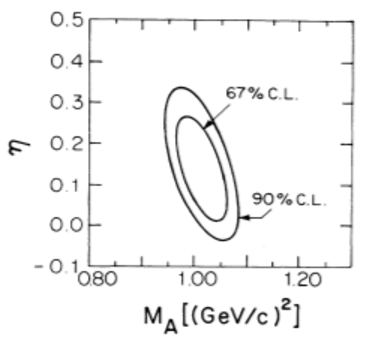
\includegraphics[angle=0,width=2.5in]{figures/intro/experiments/E734eta.pdf}
        \caption{Extracted neutral current axial form factor parameters.}
        \label{fig:e734eta}
      \end{subfigure}
      \caption{Results from the Brookhaven E734 measurement of the neutral
      current elastic cross section.}
      \label{fig:e734results}
    \end{figure}
    Figure~\ref{fig:e734xsec} shows the measured data and the cross section
    fits. Figure~\ref{fig:e734eta} shows the bounds on the axial mass $M_A$ and
    $\eta$ from the fit. In the parameter estimation, the NC axial form factor
    was assumed to have the form
    \begin{equation}\label{eq:axdipole}
      G_A^{NC}(Q^2) = \frac{1}{2}\frac{g_A}{(1+Q^2/M_A^2)^2}(1+\eta) \,,
    \end{equation}
    where $g_A$ is the weak coupling constant, $M_A$ is the axial mass, and
    $\eta$ is a factor that encodes the difference between the charged current
    axial form factor and the strange axial form factor. This form assumes that
    both parts of the form factor have the exact same shape. If the difference
    is only due to the net spin contribution of the strange quark, $\Delta s$,
    then $\Delta s = -\eta g_A$ which was found to be $-0.15 \pm 0.09$ in this
    analysis.

    A later analysis of the E734 NC elastic data was
    performed~\cite{Garvey:1992cg} in which the strange part of the electric
    and magnetic form factors was not assumed to be zero. Four fits to the
    neutrino-proton and antineutrino-proton cross section data were performed.
    In the first fit, only the axial mass was allowed to vary and the strange
    quark contribution to the electric, magnetic, and axial form factors were
    all held fixed at zero. In the second, the strange contribution to the
    electric and magnetic form factors were fixed at zero, but the axial mass
    and the strange axial form factor were allowed to vary. In the third fit,
    all three strange form factors and the axial mass were allowed to vary, and
    in the last fit, the strange form factors were all allowed to vary, but the
    axial mass was held to the world average at the time, $M_A =
    1.032\pm0.036$~GeV. The same form of the axial form factor in
    Eq.~\ref{eq:axdipole} was assumed and the strange electric and magnetic
    form factors were assumed to have the same shape as the charged current
    electric and magnetic form factors. The extracted value of $\Delta s$
    ranged from $\Delta s = -0.13 \pm 0.09$ in the second fit to $\Delta s =
    -0.21 \pm 0.10$ in the fourth fit.  Each of the extracted $\Delta s$ values
    is consistent with the original measurement and with a $\Delta s$ being
    negative.  Additionally, a strong correlation between $\Delta s$ and $M_A$
    was again observed. In the first fit with $\Delta s$ fixed at zero, a best
    fit to the data was found when $M_A = 1.086 \pm 0.015$~GeV which is very
    consistent with the original results in~\cite{Ahrens:1986xe} shown in
    Fig.~\ref{fig:e734eta}.

    An additional analysis of the E734 data considering ratios of neutral
    current elastic interactions to charged current elastic interactions was
    performed~\cite{Alberico:1998qw}. Specifically, they looked at the
    asymmetry
    \begin{equation*}
      \mathcal{A}_p(Q^2) = \frac{\Big(\frac{d\sigma}{dQ^2}\Big)_{\nu p \rightarrow \nu p} - \Big(\frac{d\sigma}{dQ^2}\Big)_{\bar{\nu} p \rightarrow \bar{\nu} p} }{\Big(\frac{d\sigma}{dQ^2}\Big)_{\nu n \rightarrow \mu^- p} - \Big(\frac{d\sigma}{dQ^2}\Big)_{\bar{\nu} p \rightarrow \mu^+ n}} \,.
    \end{equation*}
    This asymmetry has an enhancement in the strange axial and magnetic form
    factors. It was found that the experimental uncertainty was too large to
    determine $\Delta s$ and that a large factor of the uncertainty was due to
    the uncertainty on the axial mass. This analysis also assumed the dipole
    form of the axial form factor in Eq.~\ref{eq:axdipole}.

    \subsubsection{The MiniBooNE Experiment}\label{sec:miniboonence}
    The main target and detector of the MiniBooNE experiment was 800 tons of
    scintillator oil in a 12.2~m diameter spherical tank. Charged particles
    from the neutrino interactions in the mineral oil produced Cherenkov light
    which was collected by 1520 8-inch PMTs surrounding the oil. A schematic of
    the detector is shown in Fig.~\ref{fig:miniboonedetector}.
    \begin{figure}[h]
      \centering
      \includegraphics[angle=0,width=4in]{figures/intro/experiments/miniboone.png}
      \caption{Schematic of the MiniBooNE detector~\cite{Cheng:2012yy}.}
      \label{fig:miniboonedetector}
    \end{figure}
    MiniBooNE sat in the Booster Neutrino Beam (BNB) at Fermilab that can run
    in either neutrino or antineutrino mode with an average neutrino energy of
    $\sim$800~MeV~\cite{Aguilar-Arevalo:2008yp}.

    A $\Delta s$ fit to the ratio of the neutrino-proton to the
    neutrino-nucleon NC elastic cross section in the proton kinetic energy
    between $T = 350$~MeV and $T = 800$~MeV. This corresponds to a negative
    four-momentum transfer range of $Q^2 = 0.66$~GeV$^2$ to $Q^2 =
    1.5$~GeV$^2$. Figure~\ref{fig:miniboonedeltas} shows the measured ratio and
    the fits to the data.
    \begin{figure}[h]
      \centering
      \includegraphics[angle=0,width=4.5in]{figures/intro/experiments/miniboone_deltas.png}
      \caption{Ratio of the neutrino-proton NC elastic cross section to the
      neutrino-nucleon NC elastic cross section measured in
      MiniBooNE~\cite{Aguilar-Arevalo:2010cx}.}
      \label{fig:miniboonedeltas}
    \end{figure}
    In the analysis, the dipole shape in Eq.~\ref{eq:axdipole} was used for the
    axial form factor. When the value of the axial mass was held to $M_A =
    1.35$~GeV$^2$ a value of $\Delta s = 0.08 \pm 0.26$ was found, and when the
    axial mass was held to $M_A = 1.23$~GeV$^2$ a value of $\Delta s = 0.00 \pm
    0.30$. Both of these values are consistent with the E734 measurement and
    with zero.

    A later analysis of the MiniBooNE data was performed which included a
    two-body current contribution to the cross section~\cite{Golan:2013jtj}.
    The inclusion of the two-body current was done using the NuWro Monte Carlo
    neutrino event generator~\cite{Golan:2012wx}. The original MiniBooNE
    analysis used the NUANCE Monte Carlo neutrino event
    generator~\cite{Casper:2002sd}. A simultaneous extraction of $\Delta s$ and
    the axial mass from the assymetry $\mathcal{A}_p(Q^2)$ assuming the dipole
    form of the axial form factor in Eq.~\ref{eq:axdipole} and including
    two-body currents resulted in an axial mass value of $M_A =
    1.1^{+0.13}_{-0.15}$~GeV and $\Delta s = -0.4^{+0.5}_{-0.3}$. This result
    of $\Delta s$ is consistent with the original MiniBooNE result and with
    zero.

    Very recently, another re-analysis of the MiniBooNE result was performed
    using updated lattice QCD calculations of the strange electric and magnetic
    form factors and the measured MiniBooNE NC elastic nucleon cross section
    was performed~\cite{Sufian:2018qtw}. Notably, this analysis used
    z-expansion fit to the NC axial form factor (described in
    Sec.~\ref{sec:zexpansion}). A value of $\Delta s = -0.196\pm 0.127\pm
    0.041$ was found. The result was used to predict the BNL E734 NC elastic
    $\nu p$ and $\bar{\nu} p$ measurement and was found to be consistent. The
    NC elastic cross section calculated using the results are shown compared to
    MiniBooNE data in Fig.~\ref{fig:sufianuboone} and compared to E734 data in
    Fig.~\ref{fig:sufiane734}.
    \begin{figure}[h]
      \centering
      \begin{subfigure}[t]{2.5in}
        \includegraphics[angle=0,width=2.5in]{figures/intro/experiments/Sufian_MiniBooNE.png}
        \caption{Extracted NC elastic cross section compared to MiniBooNE data.}
        \label{fig:sufianuboone}
      \end{subfigure}
      \hspace{2pt}
      \begin{subfigure}[t]{2.5in}
        \includegraphics[angle=0,width=2.5in]{figures/intro/experiments/Sufian_BNL.png}
        \caption{Extracted NC elastic cross section compared to E734 data.}
        \label{fig:sufiane734}
      \end{subfigure}
      \caption{Neutral current elastic cross section results
      from~\cite{Sufian:2018qtw}}.
      \label{fig:sufiane734}
    \end{figure}

    \subsubsection{Global Fits of the Strange Nucleon Spin}


%This is the end of introduction
